\chapter{A Convolution Recurrent Neural Network}\label{chap:crnn}

In this chapter, I implement a convolutional recurrent neural network (CRNN) from the literature, train it on the \emph{pop} dataset and compare it to two baselines. I then conduct a thorough analysis of the behaviour and failure modes of the CRNN and provide motivation for improvements. 

\section{The CRNN Model}\label{sec:crnn}

I implement a convolutional recurrent neural network (CRNN) as described in \citet{StructuredTraining}, referred to as \emph{CRNN}. It remains competitive with state-of-the-art, is often used as a comparative baseline and is relatively fast and easy to train.

The model receives input of size $B \times F$ where $B=216$ is the number of bins in the CQT and $F$ is the number of frames in the song. The input is passed through a layer of batch normalisation~\citep{BatchNorm} before being fed through two convolutional layers with a rectified linear unit (ReLU) after each one. The first convolutional layer has a $5\times 5$ kernel and outputs only one channel of the same size as the input. It is intended to smooth out noise and spread information about sustained notes across adjacent frames. The second layer has a kernel of size $1\times I$ and outputs 36 channels, intended to collapse the information over all frequencies into a single 36-dimensional vector. This acts as a linear layer across frames with shared parameters for each frame. The output is passed through a bi-directional GRU~\citep{GRU}, with hidden size initially set to $256$ and a final fully connected layer with softmax activation. This produces a vector of length $C$ for each frame. The model is trained using the cross-entropy loss with the true chord distribution. The chord with the maximum probability in a frame is taken as the model's prediction.

The authors of the model also propose using a second GRU as a decoder before the final fully connected layer, called `CR2'. However, a similar effect could be achieved with more layers in the initial GRU. Furthermore, both in the paper and in brief empirical tests, the results with `CR2' were indistinguishable from the model without it. I therefore do not include this addition in model. Results left to Appendix~\ref{app:crnn_with_cr2} as they are neither relevant nor interesting.

% \subsection{Small to Large Vocabulary}

% Initial experiments were conducted on the simpler chord vocabulary with $C=25$. Only if the model could somewhat accurately classify the smaller vocabulary and if performance did not decrease using a model trained on the larger vocabulary and tested on the smaller chord vocabulary, would we proceed to using the larger vocabulary. 

% In keeping with with the methodology in \citet{StructuredTraining}, I initially run experiments using a learning rate of $0.001$. The learning rate is reduced to half its previous value if the validation loss hasn't improved for 10 epochs and training is stopped if it has not improved for 25 epochs, with a maximum of 100 epochs. Training patches of audio were set to 10 seconds long. Model convergence was manually checked using the validation and training losses over epochs.

% A plot of the training history used to ensure check convergence is shown in Figure~\ref{fig:crnn_small_vocab_loss}.

% \begin{figure}[H]
%     \centering
%     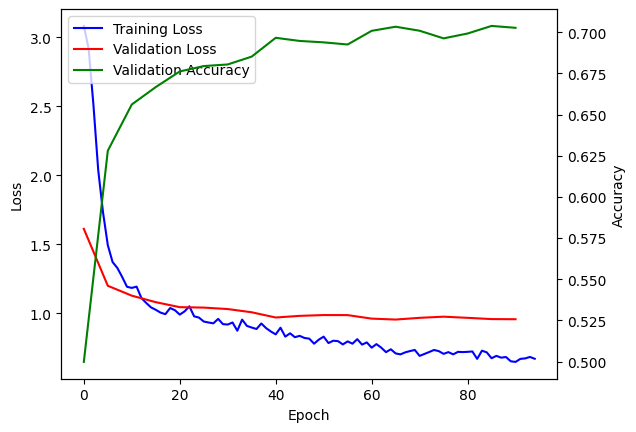
\includegraphics[width=0.8\textwidth]{figures/small_vocab_training_plot.png}
%     \caption{CRNN model training history on small vocabulary. We see the training loss and the validation loss and accuracy. The accuracy here is over all chord labels, not ignoring \texttt{X} as in final metric calculations. Training was stopped early at epoch 79. We can see the validation loss flattening out after around epoch 50. However, the model could have continued to be trained as it has not started overfitting yet. This behaviour later contributed to the argument for the removal of early stopping.}\label{fig:crnn_small_vocab_loss}
% \end{figure}

% A confusion matrix over chord roots of the model trained on $C=26$ is shown in Figure~\ref{fig:crnn_small_vocab_cm}. The model performs better than the baseline model which is tested on the larger vocabulary, which is to be expected given the nested nature of the models, and the harder task of classification with the larger vocabulary. From the confusion matrix, it becomes clear that many of the mistakes the model is making lie in the \texttt{X} symbol, which constitutes just over 7\% of the smaller vocabulary dataset. Chords with qualities like \texttt{sus4} could be confused with \texttt{major} by a reasonable model but are represented with \texttt{X} in the smaller vocabulary. Interestingly, the model trained with $C=170$ performs nearly as well on all metrics as the model trained with $C=26$. This implies that training with $C=170$ allows the model to learn almost all the relevant information about the smaller vocabulary, and gives it the chance to learn something about the larger vocabulary as well. Therefore, we proceed with the larger vocabulary for the rest of the experiments.

% While some other works continue to measure performance on the smaller vocabulary~\citep{BTC}, we believe more metrics distract from the primary goal of increasing performance across a wider range of chords. Additionally, the \texttt{third} metric captures much of the information we would look for in evaluation with $C=26$. We therefore only measure performance on the larger vocabulary from now on.

% \begin{table}[H]
%     \centering
%     \begin{tabular}{lcccccc}
%         \toprule
%         Model & $V$ for training & root & third & class\textsubscript{mean} & class\textsubscript{median} \\  
%         \midrule
%         \emph{CRNN} & 26 & 0.79 & 0.77 & 0.74 & 0.74 \\
%         \emph{CRNN} & 170 & 0.78 & 0.74 & 0.72 & 0.73 \\
%         \bottomrule
%     \end{tabular}
%     \caption{CRNN model results on the small vocabulary with $C=26$. The other metrics are omitted as they are identical to \texttt{third} for classification with $C=26$.}\label{tab:crnn_small_vocab}
% \end{table}

% \begin{figure}[H]
%     \centering
%     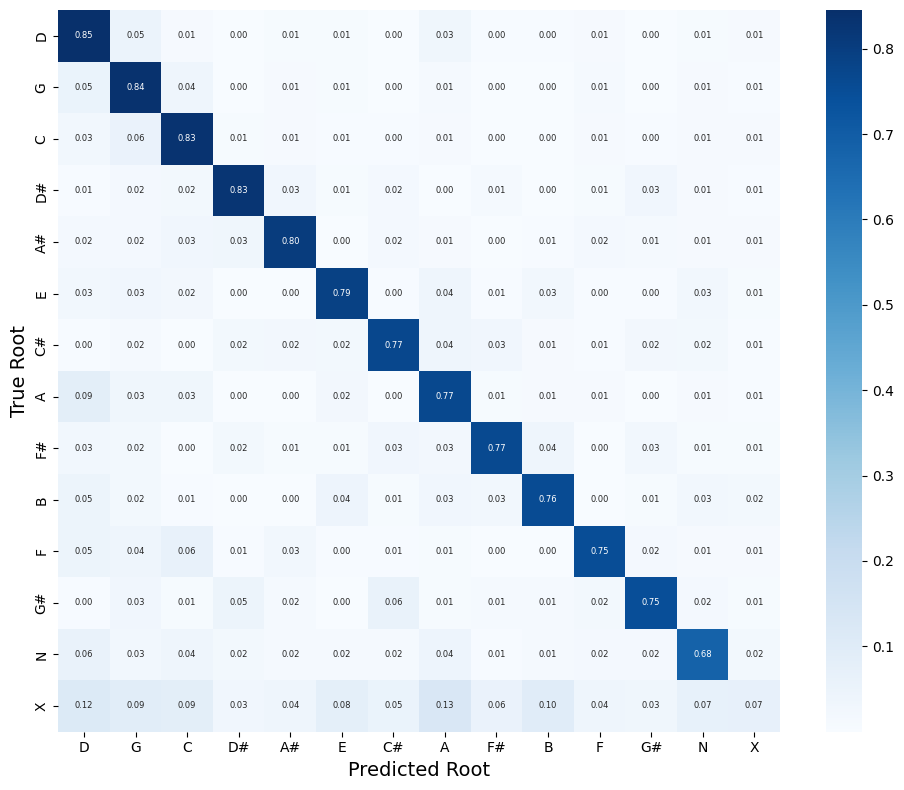
\includegraphics[width=1.0\textwidth]{figures/small_vocab_root_cm.png}
%     \caption{Confusion matrix over roots of the CRNN model trained on the small vocabulary. The values have been normalised over rows such that the values on the diagonals are recall metrics. There is a clear outlier in the model's recall with the label \texttt{X}, at just $0.07$. It also performs poorly on \texttt{N}.}\label{fig:crnn_small_vocab_cm}
% \end{figure}

\subsection{Hyperparameter Tuning}

To ensure that the training hyperparameters are set to reasonable values, I conduct a grid search over learning rates and learning rate schedulers. This is followed by a random search over model hyperparameters. 

\subsubsection{Learning rates}\label{sec:lr_search}

I perform a grid search over learning rates and learning rate schedulers in the set \texttt{[0.1, 0.01, 0.001, 0.0001]} and \texttt{[cosine, plateau, none]} respectively. \texttt{cosine} is as described in Section~\ref{sec:evaluation} and \texttt{plateau} reduces the learning rate to half its current value when validation loss has not improved for 10 epochs and stops training if it has not improved for 25 epochs.

I report a subset of metrics in Table~\ref{tab:crnn_lr}. The best performing model by validation metrics was found to be with \texttt{lr=0.001}, and very similar results over the different schedulers. I proceed with a learning rate of $0.001$ and \texttt{cosine} scheduling for the rest of the experiments. \texttt{cosine} scheduling is chosen as it provides a consistent learning rate reduction. It was empirically found that \text{plateau} sometimes only reduce the learning rate in the final epochs.

Early stopping is disabled in order to check for convergence and overfitting without the possibility of a pre-emptive stop. Judging by training graphs seen in~\ref{fig:lr_search_cosine}, the best learning rate is $0.001$. Any lower and we do not converge fast enough. Any higher and large gradient updates cause the validation accuracy to be noisy. These figures also show that the validation loss does not increase after convergence. I conclude that the model is not quick to overfit, perhaps due to the random sampling of audio patches during training. Combined with the fact that training is relatively quick and that the model is only saved on improved validation loss, I decided to remove early stopping. 

Future experiments are all conducted without early stopping, for a total of 150 epochs and with a learning rate of $0.001$ and \texttt{cosine} scheduling.

In order to check that Adam is the best optimiser to use, a training run with stochastic gradient descent (SGD) was also carried out. Results from \citet{SGD1} and \citet{SGD2} suggest that SGD can find better minima with a stable learning rate over many epochs. To test this, I trained a CRNN over 2000 epochs with a learning rate of $0.001$, the \texttt{cosine} scheduler and momentum set to $0.9$. While the model did converge, it did not perform any better than the models trained with Adam. Results are left to Appendix~\ref{app:long_sgd} for lack of interest.

\begin{figure}[H]
    \centering
    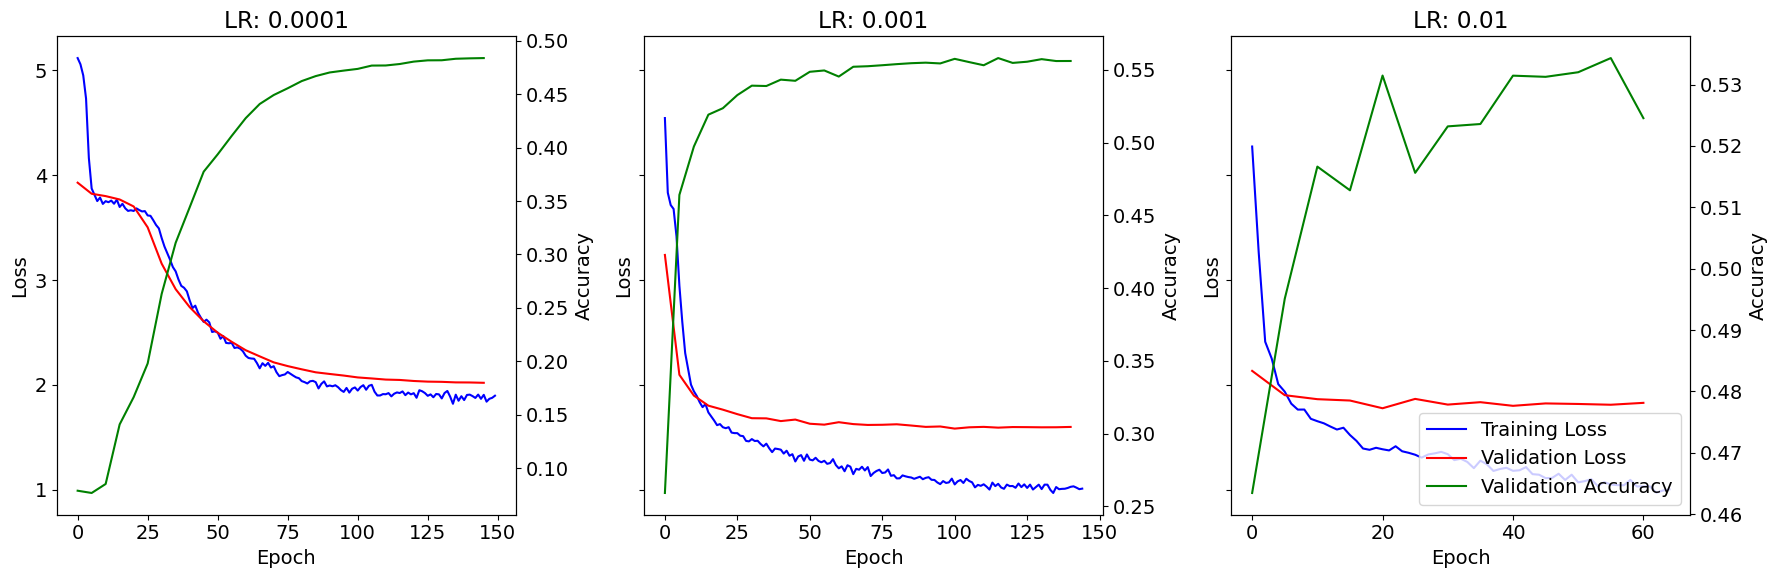
\includegraphics[width=1.0\textwidth]{figures/lr_search_cosine.png}
    \caption{Training graphs for \emph{CRNN} with different learning rates and the \texttt{cosine} scheduler. The learning rate of $0.001$ seems to be the best, as it converges in a reasonable time and the validation accuracy increases in a stable fashion. While it may seem that running for more epochs may increase performance, this was not found to be the case empirically. The best model was often achieved around epoch 100.}\label{fig:lr_search_cosine}
\end{figure}

\begin{table}[H]
    \centering
    \begin{tabular}{lcccccc}
        \toprule
        lr & scheduler & acc & root & third & seventh & mirex \\
        \midrule
        0.01 & Cosine &  53.6 & 69.5 & 66.9 & 55.7 & 78.6 \\
        0.001 & Cosine & \emph{59.7} & \emph{78.3} & \emph{75.0} & \emph{62.0} & \emph{\textbf{79.8}} \\
        0.0001 & Cosine & 53.2 & 72.1 & 66.9 & 55.2 & 72.0 \\
        \midrule
        0.001 & Plateau & \textbf{59.9} & 78.4 & 75.2 & \textbf{62.2} & 79.7 \\
        0.001 & None & 59.8 & \textbf{78.7} &\textbf{75.5} & 62.0 & 78.8 \\
        \bottomrule
    \end{tabular}
    \caption{\emph{CRNN} model results with different learning rates and schedulers. Best results over learning rates are \emph{italicised} and best results over schedulers are in \textbf{boldface}. A learning rate of $0.001$ performs the best on all metrics. The differences between learning rate schedulers are so small that the choice between them is arbitrary. }\label{tab:crnn_lr}
\end{table}

\subsubsection{Model Hyperparameters}\label{sec:model_hyperparameters}

With this learning rate and learning rate scheduler fixed, I perform a random search over the number of layers in the GRU, the hidden size of the layers in the and the training patch segment length. I also experiment increasing the number of convolutional layers prior to the GRU, the kernel size of these layers
and the number of channels outputted by each of these layers. The search is performed by independently and uniformly randomly sampling 50 points over discrete sets of possible hyperparameter values. These sets can be found in Appendix~\ref{app:random_hyperparameter_search_sets}. 

A sample of the results are shown in Table~\ref{tab:crnn_hparams}. The models were ranked according to each metric and their ranks for each metric were added up. The models were ordered by this total rank. The best model was found to have a hidden size $h=231$, a single layer GRU and a segment length of $L=23$ and the same single convolutional layer of $5\times 5$ outputting a single channel. In general, increased complexity hurts model performance but the differences between models are relatively small. Such small differences are indicative that the model is learning something simple and that increased model complexity would not help. It also seems that the choice of hyperparameters is somewhat arbitrary. The model does not utilise information from a larger context. Deeper layers with more parameters do not help performance. In fact, the parameters suggested by \citet{StructuredTraining} perform just as well as the best performing hyperparameter selection found in this random search. I therefore proceed with the same hyperparameters suggested by \citet{StructuredTraining} as default for the remainder of experiments.

\begin{table}[h]
    \centering
    \begin{tabular}{ccccccccccc}
        \toprule
        $L$ & $h$ & $k$ & $c$ & $g$ & $ch$ & acc & root & third & seventh & mirex \\
        \midrule
        23 & 231 & 5 & 1 & 1 & 1 & \textbf{59.8} & 78.2 & 74.7 & \textbf{62.0} & \textbf{79.9} \\
        11 & 150 & 7 & 2 & 1 & 3 & 59.6 & 78.5 & 75.0 & 61.9 & 79.2 \\
        43 & 222 & 11 & 2 & 2 & 2 & 59.5 & \textbf{78.7} & \textbf{75.2} & 61.8 & 78.9 \\
        \ldots & \ldots & \ldots & \ldots & \ldots & \ldots & \ldots & \ldots & \ldots & \ldots & \ldots \\
        34 & 159 & 14 & 4 & 2 & 1 & 56.9 & 75.5 & 72.2 & 59.1 & 77.7 \\
        \bottomrule
    \end{tabular}
    \caption{A subset of \emph{CRNN} model results on the large vocabulary with different hyperparameters. Best results for each metric are in \textbf{boldface}. $L$ is the length of training patches of audio in seconds, $h$ and $g$ are the hidden size and number of layers in the GRU respectively and $k$, $c$ and $ch$ are the kernel sizes, number of layers and number of channels in the CNN respectively. Models are ordered by their `Rank', calculated by adding the model's rank order over each metric, and ordering by this total. Results across most hyperparameters are very similar. Comparing with the best results from the learning rate search in Table~\ref{tab:crnn_lr}, it seems that the parameters suggested by \citet{StructuredTraining} are good choices. In general, models with more parameters and longer input tend to perform worse, perhaps due to overfitting. This suggests that the model is learning something simple.}\label{tab:crnn_hparams}
\end{table}

% Hyperparameters for CQT computation were chosen to be the same as in \citet{StructuredTraining}. However, the hop length was chosen to be $4096$ samples. Other works have used $512$ samples \citet{ACRLargeVocab1} or $2048$ samples \citet{CurriculumLearning}. It should be noted that performance is not directly comparable across hop sizes as we are changing the number of frames and so the likelihoods are different. Nonetheless, if drastically different results are obtained, it may be worth using a different hop size. A plot of accuracy against the hop size is shown in Appendix~\ref{app:accuracy_vs_hop_length}. The plot shows that performance is not affected by hop size much at all. This may be because the hop sizes used are all granular enough such that every chord has at least one frame associated with it, but not so granular that the features in a frame become too noisy. We proceed with the hop size of $4096$ samples to keep computational cost low while keeping consistent with some of the literature.


\section{Baseline Models}\label{sec:baselines}

I consider two models as baselines. First, I train a single layer neural network with softmax activation which treats each frame of each song independently. The layer receives an input of size $B=216$ outputs a $C=170$-dimensional vector for each frame. Finally, the cross-entropy loss with the true chord distribution is calculated. This model is called \emph{logistic} as it can be viewed as a logistic regression model trained using SGD. I could have used a logistic regression model implemented in \texttt{sklearn} but the implementation as a neural network was fast and easy to implement and unlikely to yield significantly different results.

% A grid search on learning rates and learning rate schedulers was conducted on the sets \texttt{[0.1, 0.01, 0.001, 0.0001]} and \texttt{[Cosine, Plateau, None]} respectively. The \texttt{Plateau} scheduler halves the learning rate when the validation loss hasn't improved for 10 epochs and \texttt{Cosine} is as described in Section~\ref{sec:training}. The best model as measured by \texttt{acc} was trained with a learning rate of $0.01$ and the \texttt{Cosine} scheduler. All models with learning rates of $0.01$ or $0.001$ converged within 150 epochs. Although the best model had a learning rate $0.01$, a learning rate of $0.001$ over 150 epochs had a more stable validation accuracy. Results are omitted for lack of interest to the main discussion. However, the search and justification of choice of model follows an identical reasoning to that followed in Section~\ref{sec:lr_search}.

Secondly, I train a convolutional neural network (CNN). The number of convolutional layers, kernel size and number of channels are left as hyperparameters. The convolutional layers operate on the CQT similarly to how a convolution operates on an image. A ReLU acts upon the activations between each layer. These convolutional layers are followed by a 36-channeled $I\times 36$ convolutional layer and fully connected layer as in \emph{CRNN}. 

I test models of increasing depths, kernel sizes and channels. In general, the deeper models perform better. Two of these models serve as baselines in reported results. The first model has a single layer and channel and a kernel size of $5$. It serves as an ablation on the GRU part of \emph{CRNN}. This configuration is referred to as \emph{CNN1}. A second model with 5 layers of kernel size 9, each with 10 channels, is referred to as \emph{CNN5}.

I performed a grid search over learning rates and schedulers for these baselines to ensure that convergence was reached. Convergence results were not meaningfully different than those obtained with the CRNN and are hence omitted. I use the best performing results in each case. This was with a learning rate of $0.001$ for both models and with schedulers of \texttt{plateau} and \texttt{cosine} for \emph{logistic} and \emph{CNN1}/\emph{CNN5} respectively.

%  The model's results can be seen in Table~\ref{tab:baseline_results}. Full results are omitted as they are not relevant to the main discussion. The model serves simply as a baseline to compare the more complex models to. These results give us the first empirical evidence that the task is non-trivial. The model is only able to predict the root of the chord with a mean frame-wise accuracy of $0.64$ and a mirex of $0.65$. The model identifies both the root and the third with an accuracy of $0.56$ but struggles more with the seventh with an accuracy of $0.44$. The lowest scores are the class-wise accuracies. The model is only able to predict the class of the chord with \texttt{class}\textsubscript{mean}$=0.13$ and \texttt{class}\textsubscript{median}$=0.03$. This gives us the first insight into each of the evaluation metrics and what we can hope from more complex models and other improvements.

% \begin{table}[H]
%     \centering
%     \begin{tabular}{lcccccccc}
%         \toprule
%         Model & frame & root & third & seventh & mirex & class\textsubscript{mean} & class\textsubscript{median} \\  
%         \midrule
%         \emph{Logistic} & 0.42 & 0.64 & 0.56 & 0.44 & 0.65 & 0.13 & 0.03 \\
%         \bottomrule
%     \end{tabular}
%     \caption{Baseline model results}\label{tab:baseline_results}
% \end{table}

\section{Results}

Table~\ref{tab:first_results} shows the results of \emph{CRNN} compared with the baseline models. \emph{CRNN} performs the best out of these models. The GRU layer improves accuracy by $5.2\%$. However, similar performance increases can be achieved by adding convolutional layers as in \emph{CNN5} rather than an RNN. Combined with the lack of performance improvement from increasing the audio patch length observed in Section~\ref{sec:model_hyperparameters}, there is strong evidence that the model does not share information across time very far.

We also observe diminishing performance increases with increased model complexity. Performance begins to level out with accuracies of only around $60\%$. Indeed, the best models trained by \citet{BTC} and by \citet{ChordFormer} never achieve an accuracy of more than $66\%$. \citet{FourTimelyInsights} refer to this as the `glass ceiling' through which the field of ACR is still struggling to break through. The problem posed by ACR is far from solved.

\citet{FeatureMaps} train a deep CNN which remains competitive with state-of-the-art to this day. It contains 8 layers. \citet{BTC} find that the performance of this deep CNN is very similar to that of \emph{CRNN}, both reaching \texttt{root} recalls between $81\%$ and $82\%$. Training much deeper convolutional networks was found to be far more computationally expensive than training \emph{CRNN}, with little performance gain to be had. Therefore, I proceed with \emph{CRNN} for further experiments.

\begin{table}[h]
    \centering
    \begin{tabular}{lccccccc}
        \toprule
        model & acc & root & third & seventh & mirex & acc\textsubscript{class} & median\textsubscript{class} \\  
        \midrule
        \emph{logistic} & 43.0 & 64.5 & 56.9 & 44.7 & 60.9 & 12.0 & 1.7 \\
        \emph{CNN1} & 54.5 & 74.4 & 69.0 & 56.6 & 73.5 & 16.0 & 2.3 \\
        \emph{CNN5} & 57.8 & 78.1 & 74.0 & 60.0 & 77.8 & 19.2 & \textbf{3.2} \\
        \emph{CRNN} & \textbf{59.7} & \textbf{78.3} & \textbf{75.0} & \textbf{62.0} & \textbf{79.8} & \textbf{19.6} & 2.3 \\
        \bottomrule
    \end{tabular}
    \caption{Results for \emph{logistic}, \emph{CNN1}, \emph{CNN5} and \emph{CRNN}. We see that \emph{CRNN} performs the best on nearly all metrics. \emph{CNN5} performs almost as well. This suggests that shallower CNNs can reach similar performance as the deep CNN trained by \citet{FeatureMaps}.}\label{tab:first_results}
\end{table}

\section{Model Analysis}\label{sec:crnn_analysis}

While quantitative metrics summarise how well a model performs over songs, they do not tell us much about the predictions the model makes and where it goes wrong. In this section, I answer several questions about the behaviour of the model.

\subsection{Qualities and Roots}

\textbf{How does the model deal with the long tail of the chord distribution?} The class-wise metrics in Table~\ref{tab:first_results} give strong indication that the performance is poor. I use a confusion matrix over qualities of chords to provide more granular detail. 

The confusion matrix is illustrated in Figure~\ref{fig:crnn_qual_cm}. The model struggles with rarer chords. On the rarest quality of majorminor7, the model has a recall of $0$. Recall is $0.86$ on the major chord but consistently predicts major for similar chord qualities like major7, major6,sus4 and sus2. A similar effect is observed on minor and similar chord qualities. The model also confuses diminished 7 chords for diminished chords. This explains the median class-wise accuracies of nearly $0$ for all models.

I also produced a confusion matrix over roots. This is left to Appendix~\ref{app:cm_roots} as it is less insightful. The model performs similarly over all roots with a recall of between $0.73$ and $0.81$. This is not surprising as the distribution over roots is relatively uniform, previously seen in Figure~\ref{fig:chord-distribution}. Recall on the no chord symbol \texttt{N} is $0.73$. Many of the \texttt{N} chords are at the beginning and end of the piece. The model may struggle with understanding when the music begins and ends. An example of the model erroneously predicting that chords are playing part-way through a song is discussed in Section~\ref{sec:crnn_examples}.

Performance is much worse on the unknown chord symbol with a recall of $0.18$. The low performance on \texttt{X} is to be expected. It is a highly ambiguous class with many very different sounds that are mapped to it. All of the chords mapped to \texttt{X} will share many notes with at least one class in the known chord portion of the vocabulary. Therefore, it is unreasonable to expect the model to be able to predict this class well. This supports the case for ignoring this class during evaluation as is standard in the literature.

\subsection{Transition Frames}\label{sec:transition_frames}

\textbf{Are predictions worse on frames where the chord changes?} Such \emph{transition frames} are present because frames are calculated based on hop length irrespective of the tempo and time signature of the song. Thus, some frames will contain a chord transition. 

To test this, I compute accuracies for transition and non-transition frames separately. The model achieves only $37\%$ on the transition frames. compared with $61\%$ on non-transition frames. Therefore, the model is certainly worse at predicting chords on transition frames. Nonetheless, \emph{CRNN} achieves an overall accuracy of $60\%$. This is because only $4.4\%$ of frames are transition frames with a hop length of $4096$. Improving performance on these frames to the level of non-transition frames would increase the overall frame-wise accuracy by much less than $1\%$. 

\begin{figure}[H]
    \centering
    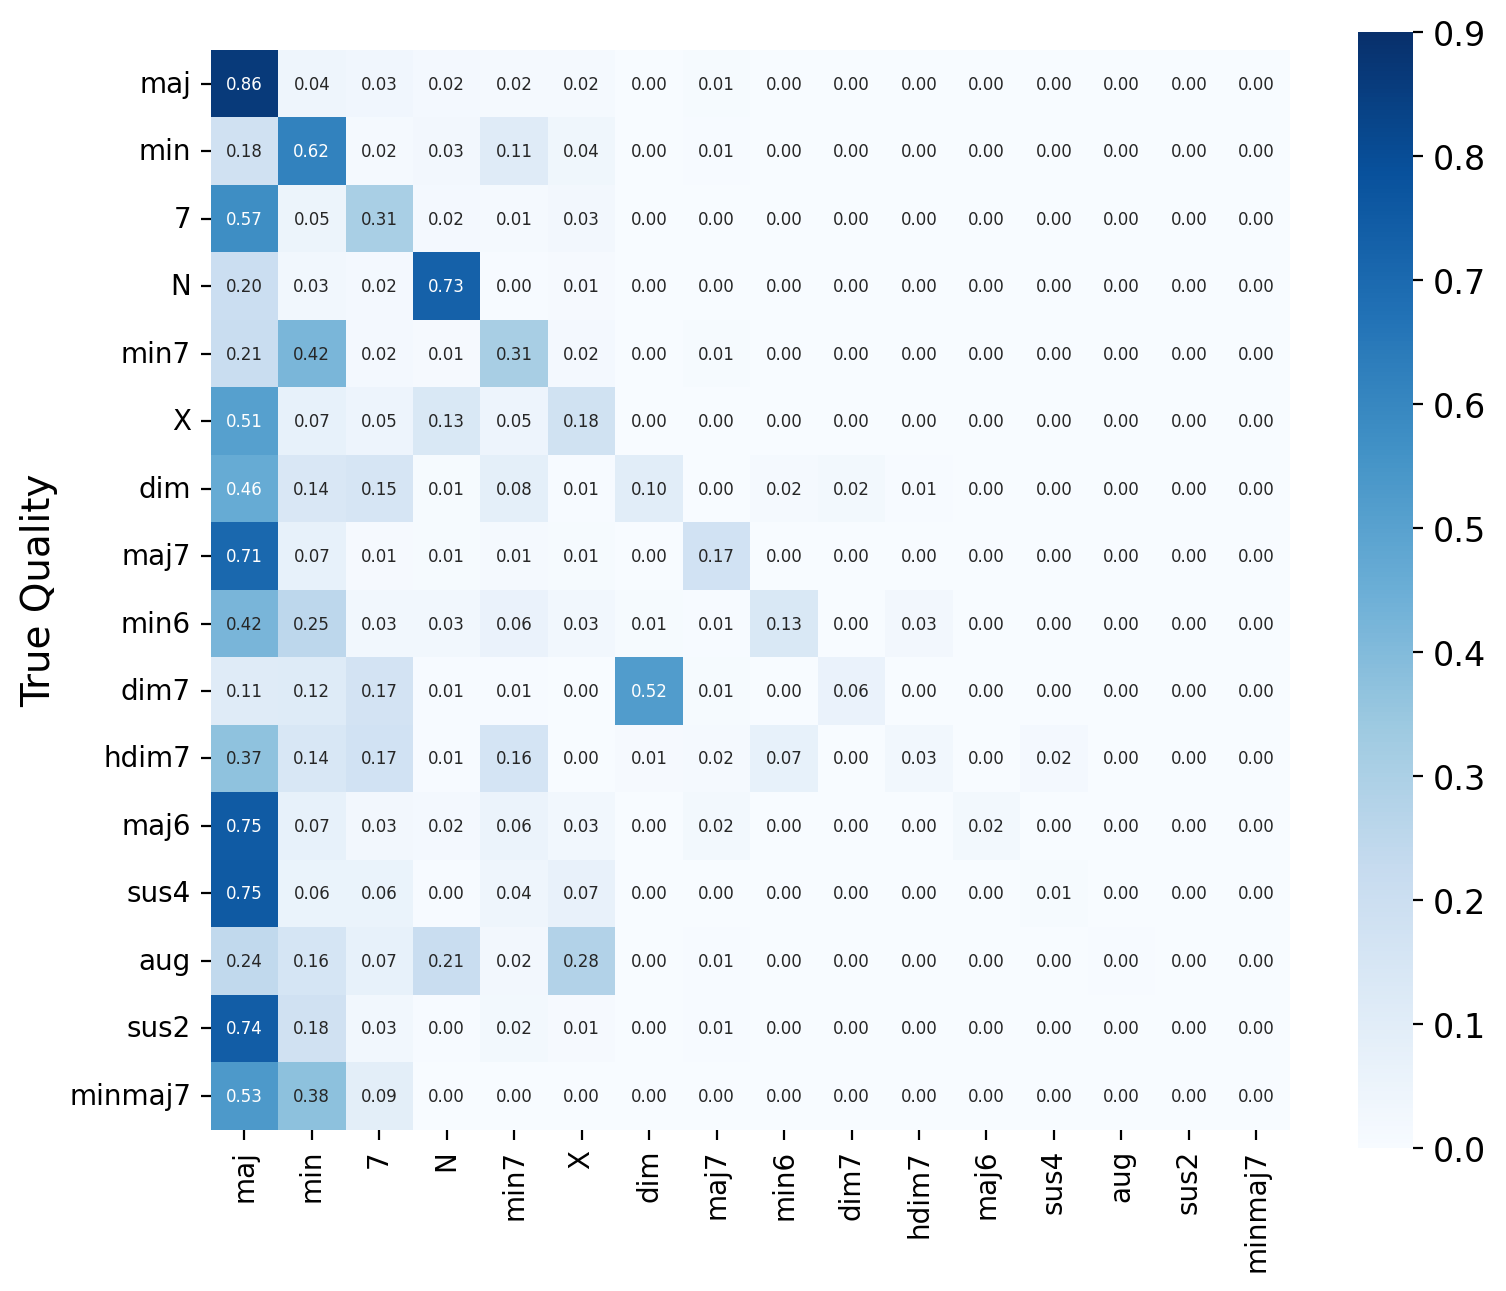
\includegraphics[width=0.9\textwidth]{figures/confusion_matrix_qualities.png}
    \caption{Row-normalised confusion matrices over qualities of the \emph{CRNN} model. Rows are ordered by frequency of chord quality. We observe that the model struggles with the imbalanced distribution. It frequently confuses \texttt{dim7} and \texttt{dim} qualities, consistently predicts \texttt{maj} for \texttt{sus2, sus4, maj6, maj7} and struggles with the two rare qualities of \texttt{minmaj7} and \texttt{aug}.}\label{fig:crnn_qual_cm}
\end{figure}

Through qualitative evaluation discussed in Section~\ref{sec:crnn_examples}, the model was found to struggle with identifying the boundary of a chord change on some songs. This would not be captured by the above metrics if the boundary is ambiguous enough to span multiple frames. Thus, there may be a larger impact in accuracy than a single frame. Furthermore, the ambiguity of chord transition timing will vary over songs. For some songs, this may be the main limiting factor in performance.

\subsection{Smoothness}\label{sec:smoothness}

\textbf{Are the models outputs smooth?} There are over 10 frames per second. If many of the model's errors are due to rapid fluctuations in chord probability, the model will over-predict chord transitions. I use two crude measures of smoothness to answer this question.

Firstly, I look at the number and length of \emph{incorrect regions}. Such a region is defined as a sequence of incorrectly predicted frames with the same prediction. $26.7\%$ of all incorrect regions are one frame wide and $3.7\%$ of incorrect frames have different predictions on either side. This can suggests that at least $3.7\%$ of errors are caused rapidly changing chord predictions. A histogram over incorrect region lengths can be found in Appendix~\ref{app:histogram_over_region_lengths}. This plot shows that distribution of lengths of incorrect regions is long-tailed, with the vast majority very short.

Secondly, I compare the mean number of chord transitions per song predicted by the model with the true number of transitions per song in the validation set. The model predicts $168$ transitions per song while the true number is $104$. This is convincing evidence that smoothing the outputs of the model could help. 

With these two observations combined, I conclude that further work on the model to improve the smoothness would might performance. Although we might hope to improve on at least $3.8\%$ of errors, this would not improve overall accuracy very much. While rapid changes may be smoothed out, there is no guarantee that smoothing will result in correct predictions. Indeed, it may even render some previously correct predictions erroneous. Nonetheless, the model is clearly over-predicting transitions in general and when being used by a musician or researcher, smoothed predictions would be valuable to make the chords more interpretable.

\subsection{Performance Across the Context}\label{sec:crnn_performance_across_context}

\textbf{How much does the model rely on context?} I hypothesise that the model is worse at predicting chords at the beginning and end of a patch of audio as it has less contextual information close to these frames. 

To test this, I evaluate the model using the same fixed-length validation conducted during training as described in Section~\ref{sec:training}. Average frame-wise accuracies over the context are then calculated. A plot can be found in Appendix~\ref{app:accuracy_over_context}. I use a segment length of $10$ seconds corresponding to $L=107$ frames. We observe that performance is worst at the beginning and end of the patch but not by much. Performance only dips by $0.05$ at either extreme, perhaps because the model still does have significant context on one side. We can also see that performance starts decreasing 5 or 6 frames from either end, suggesting this is extent to which bidirectional context is useful.

I conducted a further experiment, measuring overall accuracy with increasing segment lengths used during evaluation. Results can found in Appendix~\ref{app:accuracy_vs_context_length}. The plots show that accuracy increases by $0.5$ after increasing the segment length from 5 seconds to 60 seconds. Although this is not much of an increase, it confirms that it is better to evaluated over the entire song at once.

The predictions of the \emph{logistic} baseline use no context at all and yet achieve an accuracy of $43\%$. \emph{CNN1} only shares context a maximum of $5$ frames either side as this is its kernel size. It achieves an accuracy of $54.5$. This suggests that the majority of the performance gain associated with including contextual information is not complex nor far-reaching. Together with these experiments, I conclude that while context improves performance, it does not use context in a complex manner. 

\subsection{Consistency Over Songs}

\textbf{Does the model have consistent performance over different songs?} The set of accuracies over songs of \emph{CRNN} has a standard deviation of $13.5$. This suggests that performance is not stable over songs. To provide further insight, I plot a histogram of accuracies and \texttt{mirex} scores over the validation set in Figure~\ref{fig:crnn_song_hist}. We observe that the model has mixed performance with accuracy, with $15\%$ of songs scoring below $40\%$.  

When we use the more generous \texttt{mirex} metric, there are very few songs below $40\%$ and only $7\%$ are below $0.6$. This large discrepancy between accuracy and \texttt{mirex} suggests that many of the mistakes that the model makes are small. This mistakes are a `good guess' in the sense that the prediction may have omitted a seventh or mistaken a major 7 for its relative minor. Examples of such mistakes are discussed in Section~\ref{sec:crnn_examples}. 

I conclude that many of the model's predictions are reasonable but often lack the detail contained in good annotations like correct upper extensions. Whether these reasonable guesses are correct can vary widely over songs.

\begin{figure}[ht]
    \centering
    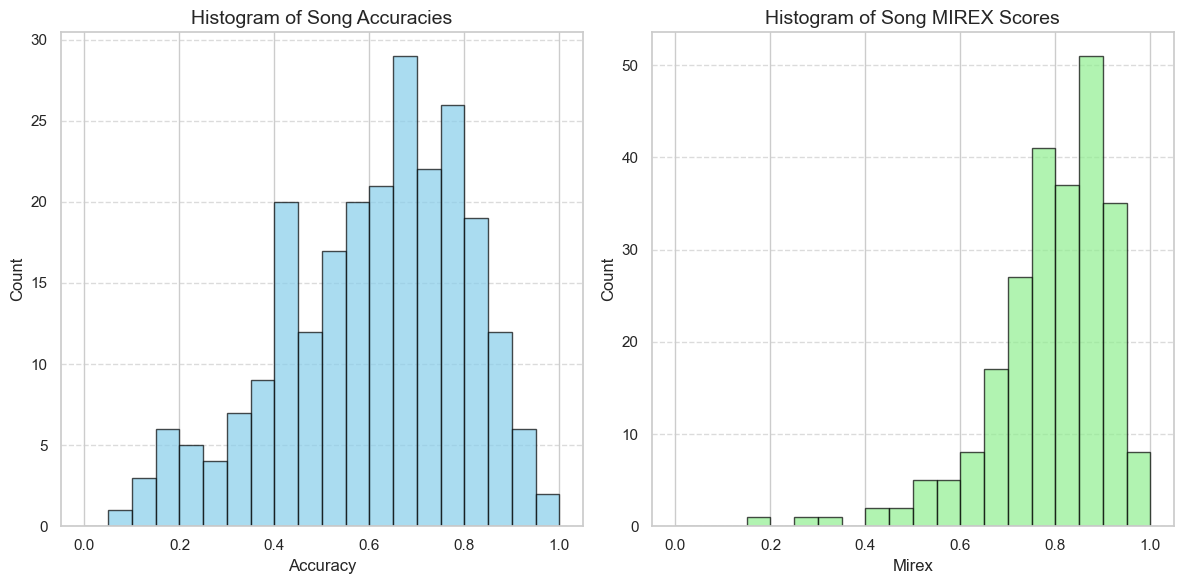
\includegraphics[width=1.0\textwidth]{figures/accuracy_mirex_histograms.png}
    \caption{Histogram of accuracies and mirex scores over songs in the validation set. Accuracies are mixed, with $15\%$ of songs below $40\%$, and $69\%$ between $0.4$ and $0.8$. However, with the more generous \texttt{mirex} metric, we find that there are almost no songs below a score of $40\%$ and only $7\%$ below $0.6$. This suggests that many of the mistakes the model makes are small, like predicting \texttt{C:maj} instead of \texttt{C:maj7}. The very low outliers in the \texttt{mirex} score were found to be songs with incorrect annotations found in Section~\ref{sec:data-integrity}.}\label{fig:crnn_song_hist}
\end{figure}

\subsection{Four Illustrative Examples}\label{sec:crnn_examples}

Let us now inspect a few songs to see how the model performs. I choose four examples showing different behaviours and failure modes of the model. Predictions are illustrated frame-by-frame and coloured by correctness, as measured by both accuracy and \texttt{mirex} score in Figure~\ref{fig:crnn_examples}. 

In `Mr.\ Moonlight', there are few differences between the accuracy and \texttt{mirex} score. There are regular repeated errors, many of which are mistaking \texttt{F:sus2} for \texttt{F:maj}. This is an understandable mistake to make, especially after hearing the song and looking at the annotation where the main guitar riff rapidly alternates between \texttt{F:maj} and \texttt{F:sus2}. The confusion matrix in Figure~\ref{fig:crnn_qual_cm} suggests this mistake is very fairly common on qualities like \texttt{sus2} which are similar to \texttt{maj}. 

In `Ain't not Sunshine', the \texttt{mirex} score is significantly higher than the accuracy. This is because the majority of the mistakes the model makes are missing a seventh. For example, the model predicts \texttt{A:min7} for the true label of \texttt{A:min7} or \texttt{G:maj} for \texttt{G:7}. Other mistakes that \texttt{mirex} allows for include confusing the relative minor or major such as predicting \texttt{E:min7} when the chord is \texttt{G:maj}. All of these mistakes occur frequently in this song. The mean difference between the accuracy and mirex is $18.7\%$, with one song reaching a difference of over $70\%$. Hence, we can attribute many of the model's mistakes to such behaviour. `Ain't no Sunshine' also contains a long incorrect section in the middle. This is a section with only voice and drums which the annotation interprets as \texttt{N} symbols but the model continues to predict harmonic content. The model guesses \texttt{A:min} throughout this section. This is a sensible label as when this melody is sung elsewhere in the song, it is labelled as \texttt{A:min7}.

In the next two songs, `Brandy' and `Earth, Wind and Fire', the model's mistakes are less interpretable. While performance is okay on `Brandy' with a \texttt{mirex} of $75.6\%$, the model struggles with the boundaries of chord changes resulting in sporadic short incorrect regions in the figure. In `Earth, Wind and Fire', the model struggles with the boundaries of chord changes and also sometimes predicts completely wrong chords which are harder to explain. Listening to the song and inspecting the annotation makes it apparent that this is a difficult song for even a human to annotate well and similarly the model does not fare well.

\begin{figure}[ht]
    \centering
    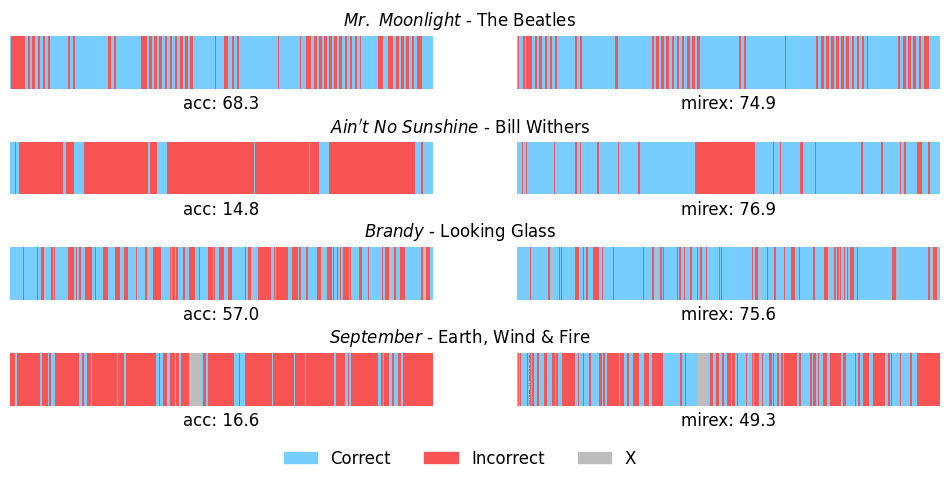
\includegraphics[width=1.0\textwidth]{figures/chord_recognition_examples.png}
    \caption{Chord predictions of the \emph{CRNN} model on four songs from the validation set (blue: correct, red: incorrect, gray: \texttt{X}). This allows us to understand some of the behaviour of the model. We can see regular repeated errors in `Mr.\ Moonlight', which are mostly mistaking two similar qualities. The discrepancy between accuracy and \texttt{mirex} on `Ain't No Sunshine' can be explained by missing sevenths in many predictions. The large incorrect region is a voice and drum only section where the model continues to predict chords due to implied harmony by the melody. Predictions in `Brandy' are quite good in general, though many errors arise from predicting the boundaries of chord changes incorrectly. The model struggles with `Earth,  Wind and Fire', missing chord boundaries, and sometimes predicting completely wrong chords. There are clearly songs where the model's outputs are less sensible. However, in general most of the model's mistakes can be explained and are reasonable.}\label{fig:crnn_examples}
\end{figure}

\section{Takeways and Next Steps}

Below, I summarise the main takeaways from this section and motivate further improvements to the model.

\textbf{Performance on rare chord classes is poor.} There are many methods of addressing an imbalanced distribution in machine learning. The simplest is to add a weighting to the loss function which I explore in Section~\ref{sec:weighted_loss}. I also look at a `structured' loss function which exploits similarity between chords in Section~\ref{sec:structured_loss}. Performance can also be improved by improving the data. I explore the use of data augmentation in Section~\ref{sec:pitch-augmentation} and synthetic data generation in Section~\ref{sec:synthetic_data}.

\textbf{Predictions are not smooth.} While it is unclear whether or not smoothness will improve performance, a good chord recognition model's predictions would be smooth. This motivates the exploration of a `decoding' step in Section~\ref{sec:decoding}. I look at using both HMMs and CRFs.

\textbf{The model does not use long-range context.} Transformers have been explored by various authors but these have not been found to increase performance. I could try to implement key estimation or genre detection as a separate component. However, in Section~\ref{sec:crnn_examples}, we saw that most of the models predictions are reasonable guesses. Its mistakes are usually subtle. Such broad information is unlikely to help much. \citet{ChorusAlignmentJAAH} explore the use of aligning choruses in jazz pieces to try to produce a single chord prediction over different sections of a piece. This is particularly suited to jazz music where different renditions of the `head' can be quite different but normally have the same underlying chords. This is not explored here. 

\textbf{The model is simple.} Outputs are often sensible but far from perfect. The feature maps analysis of a deep CNN by \citet{FeatureMaps} lines up with this idea. Their analysis suggests that the model is detecting the presence of individual notes and deciding which chord is present based on which notes it thinks are present. This is why many more parameters do not help. Unfortunately, this results in many similar chords being confused. The root note can be wrong, similar qualities are often mistaken and predictions often miss upper extension and further nuance. This explain the large discrepancy between the accuracy and \texttt{mirex} metric with average values of $79\%$ and $60\%$ over the validation set respectively. 

This problem is exacerbated by the imbalance in the dataset. There are many fewer instances of chord classes with complex qualities and upper extensions. The model ends up predicting major and minor classes for these rare chords. One method of addressing this problem is to impose some structure on the representation of the chord in order to exploit similarities between them. This is explored in Section~\ref{sec:structured_loss}.

\textbf{Chords are not interpretable in time.} The model struggles a little on transition frames. Solely improving performance on such frames is unlikely to improve metrics by much. A much better reason to segment chords is to give the output of the model a far interpretable meaning. The frame-wise correctness illustrated in Figure~\ref{fig:crnn_examples} are not musically interpretable. Even if chord symbols were added, this would not constitute good musical notation. Musicians do not operate over $93$ms frames. They think of music as existing in beat-space. \citet{AlignmentChordAnnotations} explore the related task of finding chord boundaries in audio given the chord sequence. Instead, I take inspiration from \citet{MelodyTranscriptionViaGenerativePreTraining} and use a beat detection model in order to task the model with predicting chord over beats rather than frames in Section~\ref{sec:beat-synchronisation}. 
